\documentclass[11pt,a4paper]{article}

% ─── Preamble: Packages ───────────────────────────────────────────────────────
\usepackage[utf8]{inputenc}
\DeclareUnicodeCharacter{2248}{\ensuremath{\approx}}   % “≈”
\DeclareUnicodeCharacter{2082}{\ensuremath{_2}}        % “₂”
\DeclareUnicodeCharacter{2083}{\ensuremath{_3}}        % “₃”
\DeclareUnicodeCharacter{2084}{\ensuremath{_4}}        % “₄”
\DeclareUnicodeCharacter{03BB}{\ensuremath{\lambda}}   % “λ” 
\DeclareUnicodeCharacter{03B8}{\ensuremath{\theta}}    % “θ”
\DeclareUnicodeCharacter{03BC}{\ensuremath{\mu}}       % “μ”
\usepackage[T1]{fontenc}         % modern font encoding
\usepackage{textcomp}            % extra symbols (≈, °, etc.)
\usepackage{amsmath}             % enhanced maths
\usepackage{siunitx}             % nice unit formatting
\usepackage{graphicx}            % include graphics
\usepackage{hyperref}            % clickable links
\usepackage{caption}             % caption control
\usepackage{float}               % provide [H] float specifier
\usepackage[section]{placeins}   % \FloatBarrier by section
% ─────────────────────────────────────────────────────────────────────────────

\title{EEE STAR Fundamentals of Photovoltaics Training Task 1 }
\author{İpek Cantürk \\ Department of Electrical and Electronics Engineering, METU \\ \texttt{ipek.canturk@metu.edu.tr}}
\date{\today}

\begin{document}

% ─── Cover page ───────────────────────────────────────────────────────────────
\begin{titlepage}
  \centering
  \vspace*{2cm}
  {\LARGE\bfseries EEE STAR Fundamentals of Photovoltaics Training Task 1\par}
  \vspace{1.5cm}
  {\large İpek Cantürk\par}
  {\normalsize Department of Electrical and Electronics Engineering, METU\par}
  \vspace{0.5cm}
  {\normalsize \texttt{ipek.canturk@metu.edu.tr}\par}
  {\normalsize \today\par}
  \vfill
\end{titlepage}
% ─────────────────────────────────────────────────────────────────────────────

\begin{abstract}
We evaluated ideal blackbody radiation alongside real‐world AM0 and AM1.5G solar spectra to quantify the impact of atmospheric absorption on silicon photovoltaics. Using MATLAB, we generated spectral irradiance curves for blackbodies at 300 K, 1500 K, and 6000 K via Planck’s law across 0.1–100 µm, then overlaid them with PV-Lighthouse’s AM0 and AM1.5G datasets. All plots are on log-log scale to enable better visualization. Significant absorption features—most notably the O₂ A-band near 760 nm and H₂O bands around 940 nm—cause deviations from the ideal model. By trapezoidal integration (trapz function in MATLAB) of the AM1.5G spectrum between 280–4000 nm, we found that roughly 81 percent of incident solar power exceeds silicon’s 1.12 eV bandgap, matching theoretical expectations. Our results underscore the importance of incorporating measured atmospheric spectra when modeling silicon PV performance.
\end{abstract}

\section{Introduction}
\begin{itemize}
  \item Blackbody radiation is a form of electromagnetic radiation which depends solely on the temperature of the object by which it is emitted. This idealized object is called a blackbody and it is defined as a perfect absorber and emitter of light. Blackbody radiation has a continuous spectra because it directly results from electromagnetic field formed by acceleration of electrons. Temperature dependency can in fact be viewed as a dependency on kinetic energy of electrons. The reason of continuity in field formed by accelerating electrons will not be discussed in detail in this paper as it exceeds our purpose but it is simply due to superposition of microscopic emissions.  Planck's Law describes the spectra for idealized blackbodies in a smooth curve form however, our results demonstrate important deviations from real world irradience values because actual values are affected by solar and Earth atmospheres. Understanding and assessing these effects are crucial in correct implementation of photovoltaic modelling.
  \item Planck's Law is given as follows,
  \begin{equation}
B_\lambda(T)
=
\frac{2\,h\,c^2}{\lambda^5}
\,
\frac{1}{\exp\!\bigl(\tfrac{h\,c}{\lambda\,k\,T}\bigr)\;-\;1}
\end{equation}
where Bλ(T) is the spectral radiance, h is Planck’s constant, c is the speed of light, k is Boltzmann’s constant, λ is the wavelength, T is the absolute temperature.
\end{itemize}

\section{Terminology}
\begin{itemize}
  \item Solar zenith angle is the angle between Sun rays and vertical. When the Sun is directly overhead this angle is zero and we say Sun is at zenith.
  \item Air Mass (AM) is a dimensionless quantity used to compare the path length Sun rays travel in Earth atmosphere to the path they would have traveled if at zenith.
  \item AM0 (Air Mass 0) and AM1.5G (Air Mass 1.5 Global) are Solar spectrum standards. AM0 spectrum is the solar irradience measured just before entry to Earth atmosphere. AM1.5G spectrum is the solar irradience measured at θ ≈ 48.2. This angle results in a path length 1.5 times longer than at zenith.
  \item Relation between Solar zenith angle and air mass is given by,
  \begin{equation}
  \mathrm{AM}(\theta) \;=\; \frac{1}{\cos\theta}\,,
  \label{eq:airmass}
\end{equation}
where
\[
  \theta = 0^\circ \quad\Longrightarrow\quad \mathrm{AM}=1
  \quad\text{(Sun at zenith).}
\]
  \item Electron-hole pair is the structure formed in a semiconductor when a valence electron is promotes to conduction band and thereby creates a vacancy in valence band. For electron promotion following condition must be satisfied:  
  \begin{equation}
E_{\mathrm{photon}} \;=\; h\nu \;=\;\frac{h\,c}{\lambda}
\;\ge\;E_{g}
\qquad\Longrightarrow\qquad
\lambda \;\le\;\frac{h\,c}{E_{g}}\,.
\label{eq:ehpair}
\end{equation}
Promoted electron in the conduction band acts as a negative charge carrier and hole acts as if a positive charge carrier. Under an internal electric field like a p-n junction electrons and holes are swept apart. Electrons move toward positive terminal and holes toward negative allowing current flow. When an electron falls back into a hole, the pair is recombined. This process releases energy in form of light and heat which is key to producing photocurrent and is the basis for solar cells.
  \item Bandgap is the difference in energy between the bottom of the conduction band and top of the valence band in a semiconductor. If a photon has energy lower than bandgap energy it cannot be used to form a carrier (electron hole pair). In this case it either reflects or passes through the incident surface.
\end{itemize}

\section{Methods}
\begin{itemize}
  \item Standard spectrum data is imported as raw data with 0.5 step size from PVLighthouse. There was no data available for 250-280 nm range in our data source. Therefore, we have completed the task using data from 280-4000 nm spectrum and all calculations are in accordance with this data set. 
  \item For plotting log-log scales are preferred to enable better visualization. It should be noted that this method makes data points with value zero non-visible on our graph. Important data points are marked with color-coded dots for clarity. For calculation of total irradiance and usable range by silicon we used trapezoidal integration via MATLAB’s \texttt{trapz} function .
  \item We prefered to share our scripts on Github to increase accessibility.
\end{itemize}

\section{Results}

\subsection{Blackbody Curves}
Here we compare blackbodies at different temperatures.
\begin{figure}[!htbp]
  \centering
  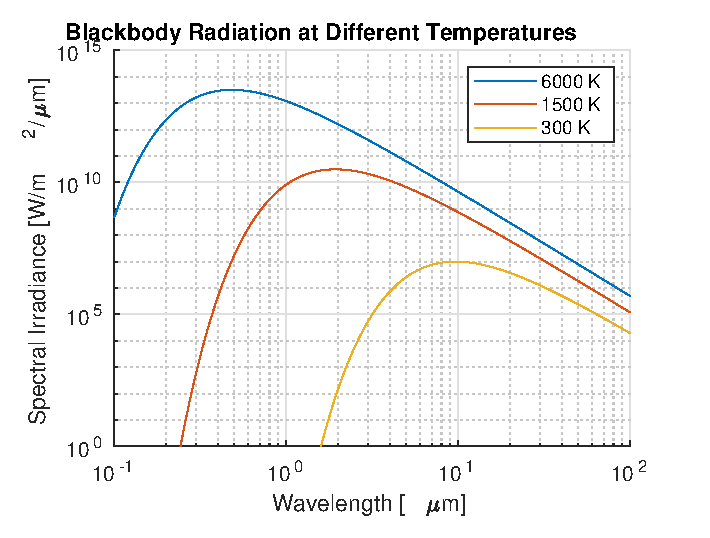
\includegraphics[width=0.8\linewidth]{blackbody_spectra.eps}
  \caption{Spectral irradiance vs.\ wavelength (0.1–100 µm) for ideal blackbodies at 300 K, 1500 K, and 6000 K, plotted on log–log axes.}
  \label{fig:blackbody}
\end{figure}

\FloatBarrier

\subsection{Solar Spectra Comparison}
Here we compare the 6000 K blackbody with the measured AM0 and AM1.5G spectra.

\begin{figure}[H]
  \centering
  \includegraphics[width=0.8\linewidth]{blackbody_vs_solar.eps}
  \caption{Comparison of the 6000 K blackbody curve with measured AM0 and AM1.5G spectra (log–log scale).}
  \label{fig:solar}
\end{figure}

\FloatBarrier

\subsection{Integrated Intensities}
\begin{itemize}
  \item Total AM1.5G (280–4000 nm): \(\approx 997.5~\mathrm{W/m^2}\).
  \item Silicon‐usable (\(\lambda \le 1108\) nm): \(\approx 805.6~\mathrm{W/m^2}\) (≈ 80.8 percent of total irradience within given spectra).
\end{itemize}

\section{Discussion}
\begin{itemize}
  \item We observe a shift in the peak towards longer wavelengths as the temperature of blackbody decreases. A blackbody at room temperature (300K) peaks near 10μm (far IR), a red hot metal blackbody (1500K) peaks near 1.9μm (near IR), and one like Sun (6000K) peaks in visible spectrum. The main reason of this phenomena is increased energy of dipole accelerators (moving electrons) with increased energy. These particles vibrate at higher frequencies. (Fig.~\ref{fig:blackbody}).  
  \item Deviation towards downward direction in AM0 data in comparison to 6000K blackbody is a resul of absorption by Sun's atmosphere. This deviation is much greater  than the one between AM0 and AM1.5G spectrums because Sun has much denser atmosphere when compared to Earth. Atmospheric absorption notches in AM1.5G result from filtering of light by atomic and molecular absorbers, and filtering by Ozone layer. Classification of absorption bands can be viewed in the table below. 
  \begin{table}[htbp]
  \centering
  \caption{Major molecular absorption bands in the AM1.5G spectrum}
  \label{tab:atm_bands}
  \begin{tabular}{@{} l l c @{}}
    \hline
    Molecule          & Band Name           & Central $\lambda$ (nm)            \\ 
    \hline
    O\textsubscript{2} & A‐band              & 759--770                          \\
    O\textsubscript{2} & B‐band              & 686--695                          \\
    H\textsubscript{2}O & Near‐IR band        & 930--960                          \\
    H\textsubscript{2}O & Overtone bands      & 1140--1200, 1400--1450, 1850--1950\\
    CO\textsubscript{2} & 1.6 µm and 2.0 µm bands & 1600, 2000                  \\
    CH\textsubscript{4} & 3.3 µm band         & 3300                              \\ 
    \hline
  \end{tabular}
\end{table}
(Fig.~\ref{fig:solar})
  \item Silicon usability is limited by bandgap; thermalization losses and absoption of usable spectra by atmospheric agents further reduce conversion efficiency.  We have found that only 80.8 \% of the standart AM1.5G spectra delivers sufficient energy to form electron-hole pairs.
\end{itemize}

\section{Conclusion}
\begin{itemize}
  \item Real spectra deviates from ideal blackbody spectra due to atmospheric effects of both the Sun and Earth. Some major molecular bands are listed in Discussion section. These bands have major effects in applications of photovoltaics as well. Oxygen A-Band reduces available photons for silicon cells by approximately 10 percent. H2O band near infrared removes can remove up to 50 \% depending on humidity, therefore humidty is a major factor of consideration when determining placement of solar farms. CO2 bands can also cause important reduction in overpolluted areas. Loses in far-infrared caused by carbondioxide and methane do not directly effect silicon cells as they are readily out of spectra. 
  \item Silicon PV can at best harvest \(\sim\)80 \% of AM1.5G power, in current cells this value is around 20-25\%.  
  \item Interactive GUI tool can be accessed at GitHub.
\end{itemize}

\section*{Code Availability}
All MATLAB scripts, raw data, instructions to reproduce these results, and the LaTeX script used to produce these report are publicly available at:  
\begin{center}
  \url{https://github.com/ipekcanturk/EEE-STAR-TASK-1}
\end{center}

\section*{Acknowledgments}
AI tools including ChatGPT o4 mini high, Claude, and Perplexity were used in writting, debugging, and optimizing the scripts used in this task.
İsmail Çınar Şahin and Mizan Karavar have contributed by providing feedback on this report and holding open discussion to enhance understanding of concepts.

\begin{thebibliography}{9}
\bibitem{Planck1901}
M.~Planck, “On the Law of Distribution of Energy in the Normal Spectrum,” \emph{Ann. Phys.}, vol.\ 4, pp.\ 553–563, 1901.
\bibitem{PVLighthouse}
“PV Lighthouse Standard Solar Spectra,” \url{https://www.pvlighthouse.com.au}, accessed May 2025.
\end{thebibliography}

\end{document}


